\subsection{Route Filtering} \label{sec:routefilter}
\begin{figure}[h!] 
	\centering
	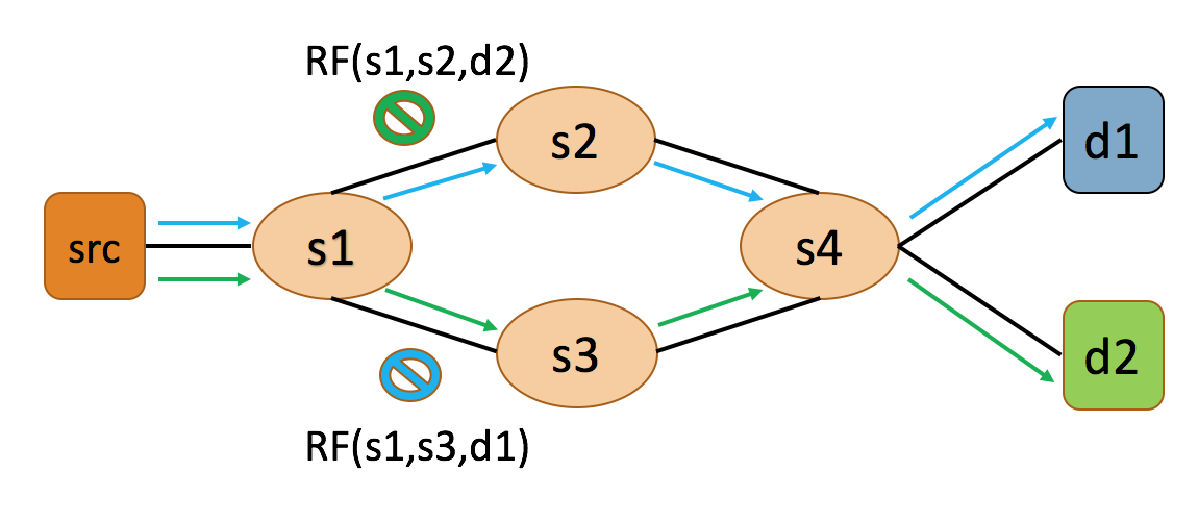
\includegraphics[width=0.8\columnwidth]{figures/diamond.eps}
	\caption{Data plane example which requires route-filtering} \label{fig:diamond}
\end{figure}
Pure ARCs cannot be synthesized for all data planes. Consider the data
plane in \Cref{fig:diamond}. 
There exists no solution to the edge weights for this data plane. 
This is because 
there are two disjoint shortest paths connecting 
$s1$ and $s4$, and each path will have 
constraints
asserting it is the shortest of the two paths. 

One way to synthesize an ARC in the scenario 
is to disable the edge
$s1 \rightarrow s3$ for destination $d1$, 
then we can synthesize ARC weights
such that path $s1 \rightarrow s2 \rightarrow s4$
 is taken to reach $d1$, 
even if the actual shortest path
from $s1$ to $s4$ is via $s2$. 
A route-filter is a mechanism 
that can be used to selectively disable
edges, as it blocks sending advertisements to a
particular destination along a link. 
Therefore, if a route-filter is added on switch $s3$, 
$s3$ 
will not advertise a route for $d1$ to $s1$, so 
$s1$ will forward to $s2$ and not to $s3$
to reach $d1$. The forwarding of packets destined
for $d2$ are not affected, and they will be sent from
$s1$ to $s4$ via $s3$ as it is the shortest path.
Thus, by incorporating route-filters, we can
disable certain links in the topology 
for specific destinations, and synthesize
ARCs for all possible data planes. 

Given a data plane, we can trivially find an 
ARC enforcing the data plane by blocking all alternate
paths by placing 
route-filters on all outgoing links other than the edges
in the DAG (e.g., disable $s1 \rightarrow s3$ for $d1$
and $s1 \rightarrow s2$ for $d2$). However, this 
ARC would be
0-resilient, and a single link failure can sever 
connectivity among endpoints (as all alternate paths
are blocked by route-filters). Thus, our objective is
to pick a set of the route-filters for each destination
such that the 
ARC satisfies certain properties. For e.g., we can
try to find the optimal number of route-filters such 
that the ARC synthesis succeeds, or we can choose a
set that maximizes the resilience of each path 
in terms of number of edge-disjoint paths in the ARC
for each endpoint. 

\Cref{fig:arcSynthesis} illustrates the synthesis of 
the ARC with route-filters. We first describe the 
modified linear equations generated when a set of
route-filters are enabled, and then describe two
techniques to choosing route-filters. 
\begin{figure}
	\centering
	\includegraphics[width=\columnwidth]{figures/arcSynthesis.eps}
	\caption{Synthesis of ARC with route-filters.} \label{fig:arcSynthesis}
\end{figure}

\minisection{Linear Equations with Route-Filters}
Given a set of route-filters, we generate a modified 
set of linear equations to satisfy the 
semantics of route-filters.
For convenience, we define $RF(sw_1, sw_2, d) = True$ 
if a route filter disables the link $sw_1 \rightarrow sw_2$
for forwarding to destination $d$ (The route filter will
actually be present on $sw_2$). 

When $RF(sw_1, sw_2, d)$ is set, we can ignore the 
weight of any path using the $sw_1 \rightarrow sw_2$
link for destination $d$, and thus 
the weight of the path of DAG $\xi_d$
starting at $sw_1$ need not be smaller than the weight
of any path
using the the $sw_1 \rightarrow sw_2$ link. Thus,
we prune \Cref{eq:uniq} to enforce the route-filter accordingly:
\begin{multline} \label{eq:uniq}
		\forall d \in \Omega. \forall s, t \in \xi_d. (s \rightarrow^+ t).\\ 
		\forall n'. (n' \in N(s) \wedge n' \not\in N(s, \xi_d) \wedge \neg RF(s,n',d)). \\
		\sum_{\mathclap{\substack{(sw_1, sw_2) \in (s \rightarrow^+ t)}}} 
		E(sw_1, sw_2) < E(s, n') + D(n', t)   
\end{multline}

If the original set of equations are inconsistent, we 
can choose a set of route-filters such that the pruned
equations become consistent. 
We discuss two schemes used to pick route-filters,
the first is finding geometrical structures called diamonds 
and the second uses unsatisfiable cores generated
by the solver.

\minisection{Diamond Elimination}
We define the structure shown in \Cref{fig:diamond}
as a \emph{diamond}. Formally,
consider two switches $s$ (the source of the diamond) 
and $t$ (the target of the diamond).
There exist two different destination DAGs with 
paths starting from $s$ such that they forward t
o different switches from $s$  
and these divergent paths from $s$ converge
at the switch $t$ first. A diamond is 
one of possible reasons for the ARC synthesis 
failing, as it forces two different paths to be 
shortest with respect to the other. 

The presence of a diamond structure is a sufficient (but not 
necessary) condition for the need of route-filters. Consider
the diamond in \Cref{fig:diamond}. There are two choices
of route-filters: the $s1-s3$ edge for destination $d1$ 
and the $s1-s2$ edge for destination $d2$, out of which,
at least one filter is required to eliminate the 
inconsistency in the linear equations caused due to the diamond.
Thus, we find all diamonds for all pairs of destination
DAGs (this is done in polynomial time) and assign a filter
to one of the two edges at the source of each diamond. 

\minisection{Unsat-Core Learning Approach}
While detecting diamonds is efficient, the
presence of diamonds is a not 
necessary condition for route-filtering.
Characterising the properties of data planes which
guarantees a pure ARC solution and thus, not requiring
route-filters, is a open algorithmic
problem. An 
efficient algorithm to find the structures causing 
inconsistencies based on these properties 
can be used to minimize the number of route-filters enabled.  

Modern LP-solvers have efficient procedures to return an
unsatisfiable core, also called IIS (Irreducible Inconsistent Subsystem)
~\cite{iis}. Formally, an IIS is a subset of constraints such that
if all constraints except those in the IIS are removed, the set of
linear equations is still inconsistent. However, further removing 
any one constraint of the IIS produces an consistent result. 

In the case of the ARC synthesis, suppose we obtain
a unsatisfiable core (unsat-core) from the solver. 
Some linear inequalities 
from \Cref{eq:uniq} will be present in the unsat-core 
(an unsat-core cannot consist only 
inequalities from \Cref{eq:dist}, as all distances set to zero
would trivially be consistent). Each linear inequality
in the unsat-core will be of the form:
\begin{eqnarray}
	\sum_{\mathclap{\substack{(sw_1, sw_2) \in (s \rightarrow^+ t)}}} 
		E(sw_1, sw_2) < E(s, n') + D(n', t)  \nonumber
\end{eqnarray}
If we set $RF(s,n',d) = True$ where the DAG of destination $d$
contains the $s \rightarrow^+ t$, then this inequality would be pruned,
and the rest of the equations in the unsat-core will be consistent (though
the complete set of equations may still be inconsistent) by the 
irreducible property of the unsat-core. By adding this route-filter
permanently to the ARC, we are assured that this unsat-core will 
never be a cause of inconsistency in our synthesis procedure. 
Thus, our unsat-core learning approach 
repeatedly extracts route-filters 
from unsat-cores to add to the ARC
till the set of equations is consistent. 

% our unsat-core learning
% approach uses the unsat-core to learn where to place a route-filter,
% and we repeat this process with an updated set of filters till the
% set of linear equations are consistent. The complete 
% algorithm of finding the set of route-filters is shown 
% in \Cref{f.

Given an unsat-core, we have a set of route-filters (obtained
from the linear inequalities of \Cref{sec:dist}) of which we 
need to choose one to eliminate this unsat-core. T
We can 
adopt a greedy approach (based on the lines of 
set cover \cite{}) of picking a route-filter which 
eliminates the maximum number of unsat-cores. However, 
finding the number of unsat-cores a route-filter eliminates
is an open problem and instrumental in minimizing the number 
of route-filters.

Alternatively, another scheme we propose in choosing route-filters
is to maximize the number of edge-disjoint paths for each pair of
endpoints in the input data plane, thus maximizing the resilience 
property of the control plane (t+1 edge-disjoint paths indicate
{\em t-resilience}). Thus, when given an unsat-core, we can choose
a route-filter which does not affect the number of edge-disjoint paths
for that pair of endpoints.

In a broad sense, the problem of synthesizing the
ARC with route-filter is as follows: given the set of all
unsat-cores for the original set of equations, find a 
set of route-filters such that each unsat-core is eliminated
by a route-filter in the set. However, we do not possess any
efficient mechanism to generate all unsat-cores. 
We are able to circumvent
this issue by finding diamonds, where each diamond corresponds
to an unsat-core and we pick a route-filter accordingly to 
eliminate them. For eliminating the 
rest of the unsat-cores, we use a solver-guided technique
to find route-filters, however there is 
great room for improvement in this approach to find the best possible
set of route-filters. 


